%%%%%%%%%%%%%%%%%%%%%%%%%%%%%%%%%%%%%%%%%
% Programming/Coding Assignment
% LaTeX Template
%
% This template has been downloaded from:
% http://www.latextemplates.com
%
% Original author:
% Ted Pavlic (http://www.tedpavlic.com)
%
% Note:
% The \lipsum[#] commands throughout this template generate dummy text
% to fill the template out. These commands should all be removed when 
% writing assignment content.
%
% This template uses a Perl script as an example snippet of code, most other
% languages are also usable. Configure them in the "CODE INCLUSION 
% CONFIGURATION" section.
%
%%%%%%%%%%%%%%%%%%%%%%%%%%%%%%%%%%%%%%%%%

%----------------------------------------------------------------------------------------
%   PACKAGES AND OTHER DOCUMENT CONFIGURATIONS
%----------------------------------------------------------------------------------------

\documentclass{article}

\usepackage{fancyhdr} % Required for custom headers
\usepackage{lastpage} % Required to determine the last page for the footer
\usepackage{extramarks} % Required for headers and footers
\usepackage[usenames,dvipsnames]{color} % Required for custom colors
\usepackage{graphicx} % Required to insert images
\usepackage{subcaption}
\usepackage{listings} % Required for insertion of code
\usepackage{courier} % Required for the courier font
\usepackage{lipsum} % Used for inserting dummy 'Lorem ipsum' text into the template

% Margins
\topmargin=-0.45in
\evensidemargin=0in
\oddsidemargin=0in
\textwidth=6.5in
\textheight=9.0in
\headsep=0.25in

\linespread{1.1} % Line spacing

% Set up the header and footer
\pagestyle{fancy}
\lhead{\hmwkAuthorName} % Top left header
\chead{\hmwkClass\ (\hmwkClassTime): \hmwkTitle} % Top center head
%\rhead{\firstxmark} % Top right header
\lfoot{\lastxmark} % Bottom left footer
\cfoot{} % Bottom center footer
\rfoot{Page\ \thepage\ of\ \protect\pageref{LastPage}} % Bottom right footer
\renewcommand\headrulewidth{0.4pt} % Size of the header rule
\renewcommand\footrulewidth{0.4pt} % Size of the footer rule

\setlength\parindent{0pt} % Removes all indentation from paragraphs

%----------------------------------------------------------------------------------------
%   CODE INCLUSION CONFIGURATION
%----------------------------------------------------------------------------------------

\definecolor{MyDarkGreen}{rgb}{0.0,0.4,0.0} % This is the color used for comments
\lstloadlanguages{Perl} % Load Perl syntax for listings, for a list of other languages supported see: ftp://ftp.tex.ac.uk/tex-archive/macros/latex/contrib/listings/listings.pdf
\lstset{language=Perl, % Use Perl in this example
        frame=single, % Single frame around code
        basicstyle=\small\ttfamily, % Use small true type font
        keywordstyle=[1]\color{Blue}\bf, % Perl functions bold and blue
        keywordstyle=[2]\color{Purple}, % Perl function arguments purple
        keywordstyle=[3]\color{Blue}\underbar, % Custom functions underlined and blue
        identifierstyle=, % Nothing special about identifiers                                         
        commentstyle=\usefont{T1}{pcr}{m}{sl}\color{MyDarkGreen}\small, % Comments small dark green courier font
        stringstyle=\color{Purple}, % Strings are purple
        showstringspaces=false, % Don't put marks in string spaces
        tabsize=5, % 5 spaces per tab
        %
        % Put standard Perl functions not included in the default language here
        morekeywords={rand},
        %
        % Put Perl function parameters here
        morekeywords=[2]{on, off, interp},
        %
        % Put user defined functions here
        morekeywords=[3]{test},
        %
        morecomment=[l][\color{Blue}]{...}, % Line continuation (...) like blue comment
        numbers=left, % Line numbers on left
        firstnumber=1, % Line numbers start with line 1
        numberstyle=\tiny\color{Blue}, % Line numbers are blue and small
        stepnumber=5 % Line numbers go in steps of 5
}

% Creates a new command to include a perl script, the first parameter is the filename of the script (without .pl), the second parameter is the caption
\newcommand{\perlscript}[2]{
\begin{itemize}
\item[]\lstinputlisting[caption=#2,label=#1]{#1.pl}
\end{itemize}
}

%----------------------------------------------------------------------------------------
%   DOCUMENT STRUCTURE COMMANDS
%   Skip this unless you know what you're doing
%----------------------------------------------------------------------------------------

% Header and footer for when a page split occurs within a problem environment
\newcommand{\enterProblemHeader}[1]{
%\nobreak\extramarks{#1}{#1 continued on next page\ldots}\nobreak
%\nobreak\extramarks{#1 (continued)}{#1 continued on next page\ldots}\nobreak
}

% Header and footer for when a page split occurs between problem environments
\newcommand{\exitProblemHeader}[1]{
%\nobreak\extramarks{#1 (continued)}{#1 continued on next page\ldots}\nobreak
%\nobreak\extramarks{#1}{}\nobreak
}

\setcounter{secnumdepth}{0} % Removes default section numbers
\newcounter{homeworkProblemCounter} % Creates a counter to keep track of the number of problems
\setcounter{homeworkProblemCounter}{0}

\newcommand{\homeworkProblemName}{}
\newenvironment{homeworkProblem}[1][Part \arabic{homeworkProblemCounter}]{ % Makes a new environment called homeworkProblem which takes 1 argument (custom name) but the default is "Problem #"
\stepcounter{homeworkProblemCounter} % Increase counter for number of problems
\renewcommand{\homeworkProblemName}{#1} % Assign \homeworkProblemName the name of the problem
\section{\homeworkProblemName} % Make a section in the document with the custom problem count
\enterProblemHeader{\homeworkProblemName} % Header and footer within the environment
}{
\exitProblemHeader{\homeworkProblemName} % Header and footer after the environment
}

\newcommand{\problemAnswer}[1]{ % Defines the problem answer command with the content as the only argument
\noindent\framebox[\columnwidth][c]{\begin{minipage}{0.98\columnwidth}#1\end{minipage}} % Makes the box around the problem answer and puts the content inside
}

\newcommand{\homeworkSectionName}{}
\newenvironment{homeworkSection}[1]{ % New environment for sections within homework problems, takes 1 argument - the name of the section
\renewcommand{\homeworkSectionName}{#1} % Assign \homeworkSectionName to the name of the section from the environment argument
\subsection{\homeworkSectionName} % Make a subsection with the custom name of the subsection
\enterProblemHeader{\homeworkProblemName\ [\homeworkSectionName]} % Header and footer within the environment
}{
\enterProblemHeader{\homeworkProblemName} % Header and footer after the environment
}

%----------------------------------------------------------------------------------------
%   NAME AND CLASS SECTION
%----------------------------------------------------------------------------------------

\newcommand{\hmwkTitle}{Project 3} % Assignment title
\newcommand{\hmwkDueDate}{Monday,\ March\ 19,\ 2018} % Due date
\newcommand{\hmwkClass}{CSC411} % Course/class
\newcommand{\hmwkClassTime}{L0101} % Class/lecture time
\newcommand{\hmwkAuthorNameone}{Yufeng Li, Yining Lin} % Your name


%----------------------------------------------------------------------------------------
%   TITLE PAGE
%----------------------------------------------------------------------------------------

\title{
\vspace{2in}
\textmd{\textbf{\hmwkClass:\ \hmwkTitle}}\\
\normalsize\vspace{0.1in}\small{Due\ on\ \hmwkDueDate}\\
\vspace{0.1in}
\vspace{3in}
}

\author{\textbf{\hmwkAuthorNameone}}
%\date{} % Insert date here if you want it to appear below your name
\date{March 19, 2018}

%----------------------------------------------------------------------------------------

\begin{document}

\maketitle
\clearpage
%----------------------------------------------------------------------------------------
%   PROBLEM 1
%----------------------------------------------------------------------------------------

% To have just one problem per page, simply put a \clearpage after each problem

\begin{homeworkProblem}
* Using Python 3.6
\\
\noindent \textit{Dataset description}
\\
The dataset contains $1968$ real news headlines and $1298$ fake news headlines. All headlines have been cleaned up by removing special characters, words from fake news that are not a part of the headline, and restricting real news headlines to those after October 2016 containing the word “trump”. This preparation is done by professor. By counting the appearance of word in real and fake news, it might predicted whether the headline is real or not, here are examples:
\\
\begin{lstlisting}[language=Python]
all_words["donald"]
{'real': 829.0, 'fake': 228.0}
all_words['trump']
{'real': 1744.0, 'fake': 1328.0}
all_words['hillary']
{'real': 24.0, 'fake': 150.0}

\end{lstlisting}

The result shows that the appearances of $trump$ and $donald$ in real news is more than the appearances in fake news, which means this word is useful for determining the headline is more likely belong to a true news. The appearances of $hillary$ indicates that the headline is likely belong to a fake news. 

\end{homeworkProblem}
\clearpage

%----------------------------------------------------------------------------------------
%   PROBLEM 2
%----------------------------------------------------------------------------------------

% To have just one problem per page, simply put a \clearpage after each problem

\begin{homeworkProblem}
We tried several combination of M and P by tuning their value in this part:
\begin{lstlisting}[language=python]
def get_prob_words_given_C(words_counts, C, num_C, m, p):
    xi_c = {}
    for word, count in words_counts.items():
        xi_c[word] = (min(count[C], num_C) + m * p) / (num_C + m)

    return xi_c
\end{lstlisting}
The result shows below:
\begin{lstlisting}
****************************
# of set:  1
M and P:  (1.0, 0.05)
Performance:  0.863265306122
****************************
# of set:  2
M and P:  (1.0, 0.1)
Performance:  0.871428571429
****************************
# of set:  3
M and P:  (2.0, 0.05)
Performance:  0.871428571429
****************************
# of set:  4
M and P:  (2.0, 0.1)
Performance:  0.881632653061
****************************
# of set:  5
M and P:  (3.0, 0.05)
Performance:  0.875510204082
****************************
# of set:  6
M and P:  (3.0, 0.1)
Performance:  0.871428571429
\end{lstlisting}
\clearpage
\begin{figure}
    \centering
    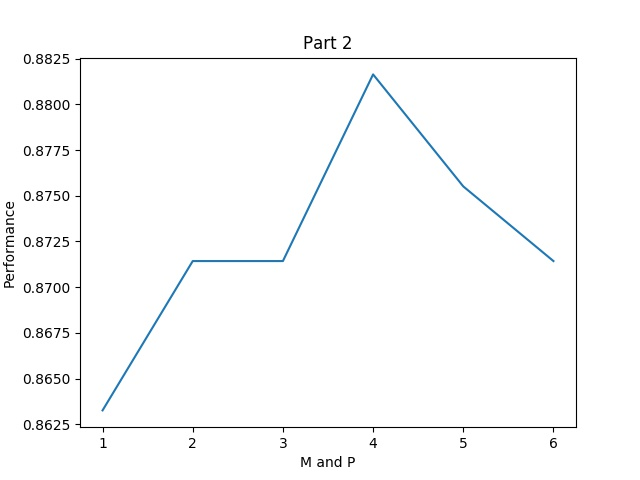
\includegraphics[scale = 0.6]{part2.jpg}
    \caption{Performance on validation set vs M and P}
    \label{fig:Performance vs M and P}
\end{figure}
According to the result, $set_6$ and $set_8$ has the best performance on validation set. We decide to use the value from set 6 in rest of the part.
\\
To deal with underflow, we simply add up all the $log(small number)$ by this function:
\begin{lstlisting}[language = python]
def get_log_sums(small_nums):
    log_sum = 0
    for small_num in small_nums:
        log_sum += np.log(small_num)
    return log_sum
\end{lstlisting}
\\
\textbf{Performance of Training set:} $0.968517708789$
\\
\textbf{Performance of Test set:} $0.848670756646$


\end{homeworkProblem}


%----------------------------------------------------------------------------------------
%   PROBLEM 3
%----------------------------------------------------------------------------------------

% To have just one problem per page, simply put a \clearpage after each problem
\begin{homeworkProblem}
\section{a)}
For words whose presence most strongly predicts that the news is real/fake, we need to use this formula:
\[
P(Condition | word) = \frac{P(word | Condition) P(Condition)}{P(word)}
\]

For words whose absence most strongy predicts that the news is real/fake, we use this formula:
\[
P(Condition | not\ word) = P(Condition | all\ words) - P(Condition | the\ word)
\]
\\
By applying to the formula above, we have all the probabilities storing in four dictionaries regarding to each word. The result showing below are the top 10 words with highest probabilities in each dictionary. 
\\
\textbf{List the 10 words whose presence most strongly predicts that the news is real.}
\[
['trump', 'donald', 'to', 'us', 'on', 'trumps', 'in', 'of', 'for', 'says']
\]

\textbf{List the 10 words whose absence most strongly predicts that the news is real.}
\[
['ron', 'neocons', 'watch', 'shameless', 'instantly', 'regrets', 'fleeing', 'dreams', 'secrecy', 'faked']
\]

\textbf{List the 10 words whose presence most strongly predicts that the news is fake.}
\[
['trump', 'the', 'to', 'in', 'donald', 'for', 'of', 'a', 'and', 'on']
\]

\textbf{List the 10 words whose absence most strongly predicts that the news is fake.}
\[
['glass', 'snl', 'skit', 'korea', 'awkward', 'handshakes', 'g20', 'agenda', 'scouts', 'aides']
\]
\\
\textbf{Influence of Presence vs Absence} \\
We compare the performance of presence and absence word by swapping the probabilities of top 10 presence word and top 10 absence word for both real and fake. Here is the result:
\begin{lstlisting}
presence->absence:
training accuracy: 0.881504153913
validating accuracy: 0.728571428571
testing accuracy: 0.760736196319
\end{lstlisting}
\\
Replace all the probabilities of top 10 absence word to top 10 presence word.
\begin{lstlisting}
absence->presence:
training accuracy: 0.908613904679
validating accuracy: 0.787755102041
testing accuracy: 0.775051124744
\end{lstlisting}
\\The original performance is:
\begin{lstlisting}
naive bayes summary:
training accuracy: 0.964145168343
validating accuracy: 0.881632653061
testing accuracy: 0.852760736196
\end{lstlisting}
\\We can see that when presence top words becomes absence that performance drop is greater than that of absence top word becomes presence. So presence words have a stronger say in the prediction.




\section{b)}
After removing stop words from dictionaries, we get the result below:
\\
\textbf{10 non-stopwords that most strongly predict that the news is real.}
\[
['trump', 'donald', 'trumps', 'says', 'north', 'election', 'korea', 'clinton', 'ban', 'russia']
\]
\\
\textbf{10 non-stopwords that most strongly predict that the news is fake.}
\[
['trump', 'donald', 'hillary', 'clinton', 'election', 'just', 'new', 'america', 'president', 'obama']
\]
\section{c)}
Stop words such as $about$ and $above$ should be count as neutral words, which will not contribute to classifying whether the headline is true or not. 
\end{homeworkProblem}
\clearpage



%----------------------------------------------------------------------------------------
%   PROBLEM 4
%----------------------------------------------------------------------------------------

% To have just one problem per page, simply put a \clearpage after each problem

\begin{homeworkProblem}
By trying different combination of $\alpha$ and $\lambda$(i.e. the regularization factor), we find out that the best $\lambda$ should be $\frac{1.0}{Number\ of\ samples}$. The value of $\alpha$ is a common value for regularization. 
\\
 We choose to use $pytorch$ to construct and train the model, and using L2 regulation to avoid overfitting because we derived test using L1,L2 regularization and the performance of testing set is:
\\
L2 Regularization accuracy: 0.828220858896
\\
L1 Regularization accuracy: 0.820040899796
\\It is obvious that we'd better use L2 regularization.
\begin{figure}[!ht]
    \centering
    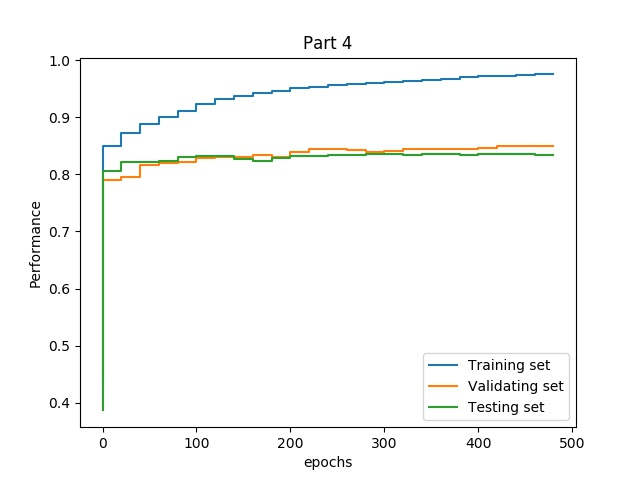
\includegraphics[scale = 0.8]{part4.jpg}
    \caption{Epochs VS Performance}
\end{figure}
\\
By using the values below, we get the curve in $Figure 2$
\\
$\alpha: 1e-2$
\\
\lambda: \frac{1.0}{Number\ of\ samples}
\\$L2 regularization(i.e. train\_l2() in logistic.py)$

\end{homeworkProblem}
\clearpage

%----------------------------------------------------------------------------------------
%   PROBLEM 5
%----------------------------------------------------------------------------------------

% To have just one problem per page, simply put a \clearpage after each problem

\begin{homeworkProblem}
\\
\textbf{Naive Bayes}
\\
$\theta_0: P(C)$
\\
$\theta_i: 1$
\\
$I(x): \frac{count(x_i=1,C) + mp}{count(C) + m}$
\\\\
\textbf{Logistic Regression}
\\
$\theta_0$: bias
\\
$\theta_i$: weight\ of\ each\ word
\\
  I(x)=\left\{
  \begin{array}{@{}ll@{}}
    1, & \text{if}\ word\ appears \\
    0, & \text{otherwise}
  \end{array}\right.


\end{homeworkProblem}

%----------------------------------------------------------------------------------------
%   PROBLEM 6
%----------------------------------------------------------------------------------------

% To have just one problem per page, simply put a \clearpage after each problem

\begin{homeworkProblem}
We use one hot encoding to indicate real$(1,0)$ and fake$(0,1)$, thus every $\theta$ is a vector with length equal to 2.
\section{a)}
\textbf{For Real Label}
\\
Top 10 positive $\theta$
\[
['trumps', 'turnbull', 'trump', 'us', 'says', 'donald', 'korea', 'debate', 'ban', 'north']
\]
Top 10 negative $\theta$
\[
['hillary', 'breaking', 'watch', 'just', 'america', 'victory', 'new', 'are', 'they', 'the']
\]
\textbf{For Fake Label}
\\
Top 10 positive $\theta$
\[
['hillary', 'breaking', 'watch', 'just', 'america', 'victory', 'new', 'are', 'they', 'the']
\]
Top 10 negative $\theta$
\[
['trumps', 'turnbull', 'trump', 'us', 'says', 'donald', 'korea', 'debate', 'ban', 'north']
\]
\textbf{Comparing list of word between part3a and part6a}
\\
The list in part3a has more $STOP WORD$ such as $to$ and $on$ comparing to the list in part6a. There are some common words in both list such as $trump$ and $says$. 
\\
\section{b)}
After removing all stop words
\\
\textbf{For Real Label}
\\
Top 10 positive $\theta$
\[
['trumps', 'turnbull', 'trump', 'says', 'donald', 'korea', 'debate', 'ban', 'north', 'comey']
\]
Top 10 negative $\theta$
\[
['hillary', 'breaking', 'watch', 'just', 'america', 'victory', 'new', 'voter', 'star', 'supporter']
\]
\textbf{For Fake Label}
\\
Top 10 positive $\theta$
\[
['hillary', 'breaking', 'watch', 'just', 'america', 'victory', 'new', 'star', 'voter', 'supporter']
\]
Top 10 negative $\theta$
\[
['trumps', 'turnbull', 'trump', 'says', 'donald', 'korea', 'debate', 'ban', 'north', 'comey']
\]
\\
\textbf{Comparing list of word between part3b and part6b}
\\
There are some common words in both list such as $donald$ and  $hillary$. By comparing the rank of the same word in different list, it shows that the two algorithm using different way to weight them.
\section{c)}
We don't compare magnitude in regression. For example, assume there is a big magnitude and a small magnitude, they contribute the same for the outcome. It is incorrect to use importance to conclude the comparison. For Logistic Regression, we only focus on whether something happen or not, not their time of occurrence.
Because the coefficient is useful to formulate into formulas, thus we can plug the input to get prediction. 

\end{homeworkProblem}
\clearpage
%----------------------------------------------------------------------------------------
%   PROBLEM 7
%----------------------------------------------------------------------------------------

% To have just one problem per page, simply put a \clearpage after each problem

\begin{homeworkProblem}
\section{a)}
    Show the relationship between the $max\_depth$ of the tree, and the training / validation accuracy
    \begin{figure}[!ht]
    \centering
    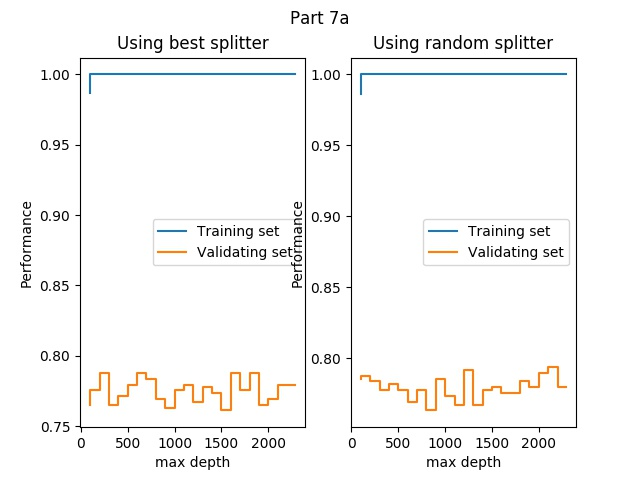
\includegraphics[scale = 0.8]{part7a.jpg}
    \caption{Maxdepth VS Performance(generated using $>$20 different max depths)}
    \end{figure}
    \\Here I applied different splitter to see their performance, overall best splitter has a better outcome
    \begin{lstlisting}
    best maxdepth for best splitter: 200
    its validating performance: 0.787755102041
    best maxdepth for random splitter: 400
    its validating performance: 0.779591836735
    \end{lstlisting}
    \\Also, it appears that best splitter acquires smaller max depth thus a faster training.
    \\Finally, the code I'm using to train decision tree:
    \begin{lstlisting}
    tree.DecisionTreeClassifier(splitter='best', presort=True, max_depth=200,/
    criterion='entropy')
    \end{lstlisting}
    \\According to sklearn documents, presort can speed up the training and we are using entropy here to train.
    
\section{b)}
The code I use to generate visualization:
\begin{lstlisting}
import graphviz
from subprocess import call
clf = train(train_x, train_y, 200, 'best')
tree.export_graphviz(clf, out_file='tree.dot', feature_names=words_order, max_depth=3,/
class_names=['fake', 'real'])
call(['dot', '-Tpng', 'tree.dot', '-o', 'tree.png'])
\end{lstlisting}
\\And I extracted the top three levels of the tree:
\begin{figure}[!ht]
    \centering
    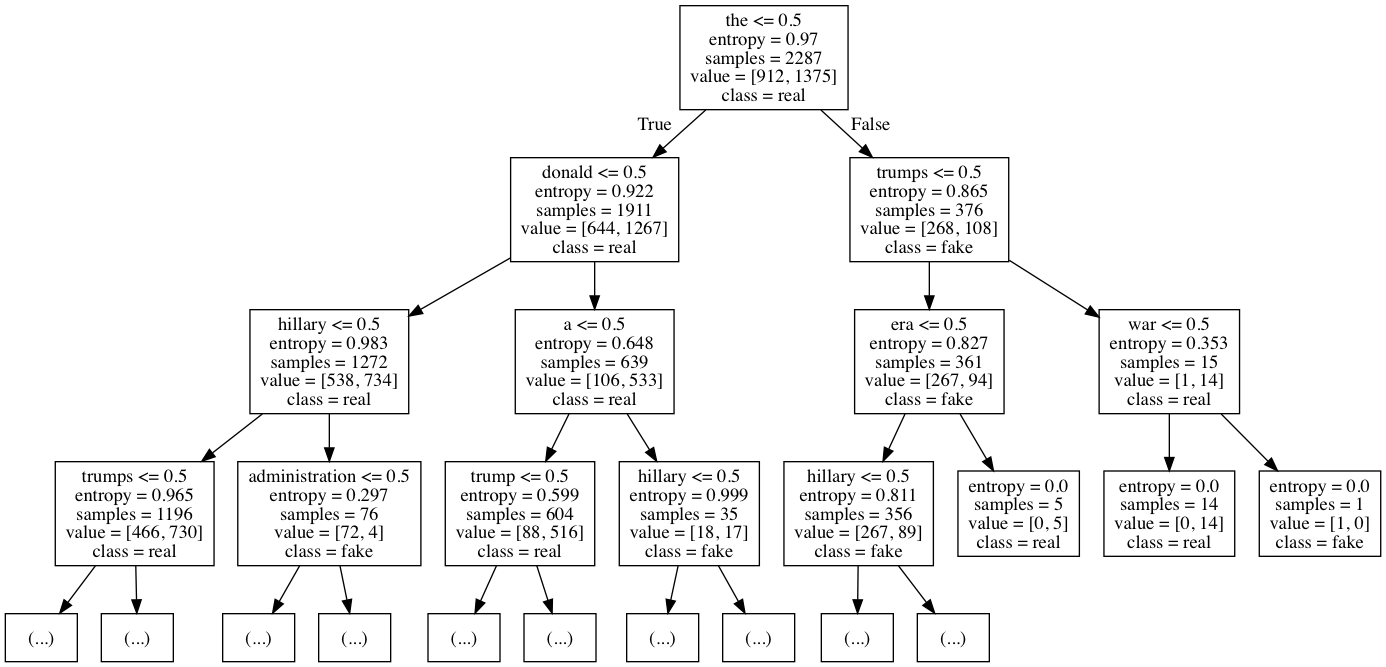
\includegraphics[scale = 0.35]{tree.png}
    \caption{Top 3 level of trained decision tree}
    \end{figure}
\\I noticed that the most important features was:
\[
['the', 'donald', 'trump', 'hillary', 'a', 'era', 'war', 'trumps', 'administration']
\]
It shares some similarity with both of them. Some of the most importance feature appeared in top 10 positive/negative $\theta$ of logistic regression or most strong presence/absence of naive bayes. This indicates that those words are very important to determine in these three methods of classification.

\section{c)}
The performance summaries of three classifications are:
\begin{lstlisting}
naive bayes summary:
training accuracy: 0.964145168343
validating accuracy: 0.881632653061
testing accuracy: 0.852760736196

logistic regression summary:
training accuracy: 0.946217752514
validating accuracy: 0.834693877551
testing accuracy: 0.826175869121

decision tree summary:
training accuracy: 1.0
validating accuracy: 0.781632653061
testing accuracy: 0.768916155419
\end{lstlisting}
\\Overall, I would say naive bayes' performance is relatively the best and train faster than logistic regression but a little bit slower than decision tree, presumably because I heavily used dictionary in naive bayes training which maybe slower than building tree using sklearn. I would expect it to be much faster using vectorized code.

\end{homeworkProblem}
\clearpage

\begin{homeworkProblem}
\section{a)}
I use following code to get the first split data:
\begin{lstlisting}
def random_train_top(x, y, maxweights):
    clf = tree.DecisionTreeClassifier(splitter='best', max_depth=1, /
    criterion='entropy', max_features=maxweights)
    clf = clf.fit(x, y)
    return clf
\end{lstlisting}
\\Then I used the same method the produce the tree structured graph:
\begin{lstlisting}
import graphviz
from subprocess import call
clf = random_train_top(train_x, train_y, 100)
tree.export_graphviz(clf, out_file='tree0.dot', feature_names=words_order, max_depth=1,
                         class_names=['fake', 'real'])
call(['dot', '-Tpng', 'tree0.dot', '-o', 'tree0.png'])
\end{lstlisting}
\\Which produce a decision tree:
\begin{figure}[!ht]
    \centering
    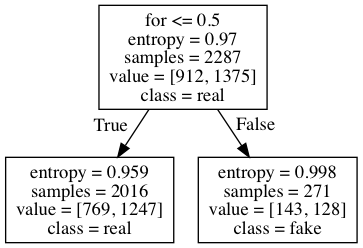
\includegraphics[scale = 0.8]{tree0.png}
    \caption{decision tree to compute I(Y,'for')}
    \end{figure}
\\Here's how I compute:
\\Y=['fake','real']
\\
\\H('for')=-(912/(912+1375))*log_2(912/(912+1375))-(1375/(912+1375))*log_2(1375/(912+1375))=0.9702
\\
\\H('for'|Y)=(((769+1247)/(2287))*(-(769/(769+1247))*log2(769/(769+1247))-(1247/(769+1247))*log2(1247/(769+1247))))+(((143+128)/(2287))*(-(143/(143+128))*log2(143/(143+128))-(128/(143+128))*log2(128/(143+128))))=0.9636
\\
\\I(Y,'for')=0.9702-0.9636=0.0066
\section{b)}
\\Similarly, using the above code, I generated another decision tree with a different $x_j='a'$:
\begin{figure}[!ht]
    \centering
    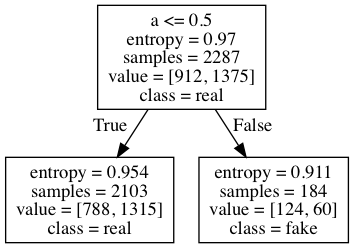
\includegraphics[scale = 0.8]{tree1.png}
    \caption{decision tree to compute I(Y,'for')}
    \end{figure}
\\Here's how I compute:
\\Y=['fake','real']
\\
\\H('a')=-(912/(912+1375))*log_2(912/(912+1375))-(1375/(912+1375))*log_2(1375/(912+1375))=0.9702
\\
\\H('a'|Y)=(((788+1315)/(2287))*(-(788/(788+1315))*log2(788/(769+1315))-(1315/(788+1315))*log2(1315/(788+1315))))+(((124+60)/(2287))*(-(124/(124+60))*log2(124/(124+60))-(60/(124+60))*log2(128/(124+60))))=0.9175
\\
\\I(Y,'a')=0.9702-0.9175=0.0527
\\
\\$In conclusion, I(Y,'a') is bigger than I(Y,'for') which indicates we can learn more information by using 'a' as split thus its better$

\end{homeworkProblem}
\clearpage




\end{document}